% Extensión estimada: unas 4 páginas, dos subsecciones, dos tablas y una figura (ficha 5.4).
% Fuentes: cap5_derivados.json ("entre_generadores", "fallas": cobertura, palabras y reportes distintos con Swin-Tiny);
% ensemble_bootstrap*_les_report_only_strict.json; Codigo/docs/resul/mini_vlm_lora_llm_resul_v3_20261024.md (control,
% parcial: Swin-Tiny 963 de 1 503, sin anclaje 372); cost/cost_comparison_v3.json (segundos por reporte, de las
% corridas del re-anclaje en la A30; parámetros); logs 1153597 y 1153598 (segunda etapa: 9 h 21 min y 6 h 55 min).
% Memoria y parámetros medidos en la A30: cost/vlm_memory_<gen>.json (scripts/measure_vlm_memory.py, Mendieta
% 1183335–37; torch.cuda.max_memory_allocated en GiB, 20 reportes de la cascada). Nivel 1 pareado de la variante de
% control: level1_test/skincot_test_mini_v2/level1_pareado_mini_v2_v3_llava_v2.json (n = 349).
% Figura: scripts/figuras_cap5.py (resumen-generadores).
% El label del costo es sec:res_costo (lo cita el Capítulo 6).
\section{Comparación entre los generadores}
\label{sec:res_gen_comparacion}

Las secciones anteriores siguieron sobre todo a Mini-VLM, la configuración principal, y mencionaron a los otros
generadores donde se comportan distinto. Puestos en una misma escala, la Figura~\ref{fig:res_gen_resumen} reúne lo que
separa a los tres con el diagnóstico de Swin-Tiny: la consistencia diagnóstica, la cobertura de entidades clínicas y el
tiempo por reporte.

\begin{figure}[H]
    \centering
    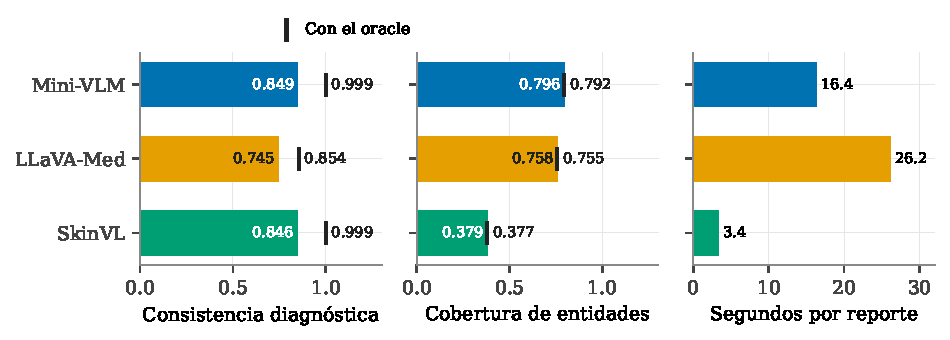
\includegraphics[width=\textwidth]{Figures/Capitulos/05-Resultados-Generacion/resumen-generadores.pdf}
    \caption{Consistencia diagnóstica, cobertura de entidades clínicas y tiempo por reporte de los tres generadores
    en la cascada con Swin-Tiny. La marca vertical es la consistencia con el \emph{oracle}.}
    \label{fig:res_gen_resumen}
\end{figure}

En consistencia, Mini-VLM y SkinVL no se distinguen, ni con Swin-Tiny ni con el \emph{oracle}, porque los dos copian el
diagnóstico. Mini-VLM supera a LLaVA-Med por una décima con Swin-Tiny, 0.104 [0.087, 0.122], y la diferencia crece con
el \emph{oracle}, porque en ese caso todas las fallas son del generador. Es decir, el generador biomédico más grande es
el que menos transcribe el diagnóstico recibido.

La cobertura de entidades separa a SkinVL de los otros dos. Sus reportes tienen una mediana de 17 palabras, frente a 62
de Mini-VLM y 86 de LLaVA-Med, y cubren la mitad de las entidades clínicas. Además, con Swin-Tiny escribe solo 59
reportes distintos para las 1\,503 imágenes, de modo que su texto depende del diagnóstico y casi nada de la imagen. Por
lo tanto, la especialización en dermatología no mejora la fidelidad del reporte, que ya fija el clasificador, y reduce
la descripción, que es lo que el generador agrega en la cascada. Mini-VLM, en cambio, iguala la fidelidad de SkinVL y
describe tanto como LLaVA-Med, y por eso es el generador de referencia del trabajo.

\subsection{Ajuste del modelo de lenguaje de Mini-VLM}
\label{sec:res_gen_control_mini}

En la configuración principal, Mini-VLM aprende a redactar sin que se ajuste su modelo de lenguaje
(Sección~\ref{sec:met_generacion}). La variante de control, que también ajusta ese modelo, permite saber si esa
decisión cambia los reportes. La Tabla~\ref{tab:res_gen_control} compara ambas versiones sobre las mismas imágenes en
cada fuente de diagnóstico; en la cascada con Swin-Tiny y sin anclaje, la variante de control tiene reportes solo para
una parte de la prueba.

\begin{table}[H]
    \centering
    \caption{Consistencia diagnóstica de la variante de control de Mini-VLM frente a la configuración principal, con
    IC del 95\,\% (\emph{bootstrap} pareado).}
    \label{tab:res_gen_control}
    \small
    \begin{tabularx}{\textwidth}{@{}>{\raggedright\arraybackslash}X cccc@{}}
        \toprule
        \textbf{Fuente del diagnóstico} & \textbf{Imágenes} & \textbf{Control} & \textbf{Principal}
            & \textbf{Diferencia} \\
        \midrule
        \emph{Oracle} & 1\,503 & 0.967 & 0.999 & $-0.033$ [$-0.042$, $-0.023$] \\
        Swin-Tiny & 963 & 0.843 & 0.850 & $-0.007$ [$-0.021$, $+0.006$] \\
        Sin anclaje & 372 & 0.196 & 0.185 & $+0.011$ [$-0.043$, $+0.065$] \\
        Nivel diferencial & 248 & 0.863 & 0.831 & $+0.032$ [$-0.008$, $+0.077$] \\
        \bottomrule
    \end{tabularx}
\end{table}

Ajustar el modelo de lenguaje no cambia la cascada con Swin-Tiny ni el nivel diferencial, y en la generación sin
anclaje tampoco mejora la consistencia. Lo que sí cambia es el formato: la variante de control aprende la estructura de
\emph{SkinCoT} y abre bloques de razonamiento en uno de cada cuatro reportes de \emph{HAM10000}. Con el \emph{oracle},
esa estructura le cuesta tres centésimas de consistencia, porque en parte de los reportes el límite de 384 tokens llega
antes de que el diagnóstico salga del razonamiento.

En \emph{SkinCoT}, el mismo efecto es mayor. La variante de control abre un bloque de razonamiento en casi dos de cada
tres reportes, y uno de cada seis queda vacío al quitarlo. Sobre los 349 pares en que ambos generadores escriben un
reporte, además, el parecido con la referencia cambia poco y en sentidos opuestos según la métrica: la variante de
control supera a la principal en BLEU-4 y en BERTScore, 0.781 frente a 0.770, y queda por debajo en ROUGE-L y METEOR,
mientras que las dos quedan por debajo de LLaVA-Med en las cinco. Por lo tanto, ajustar el modelo de lenguaje acerca el
formato al de \emph{SkinCoT} sin mejorar la fidelidad ni, de manera consistente, el parecido con la referencia, a
costa de reportes vacíos, y la configuración principal se mantiene.

\subsection{Costo computacional del pipeline}
\label{sec:res_costo}

El costo de los clasificadores, que se mide en milisegundos por imagen (Sección~\ref{sec:res_costo_clasificadores}),
es una parte mínima del costo del \emph{pipeline}. La Tabla~\ref{tab:res_costo_generadores} reúne el de los
generadores: el tiempo del ajuste, el tiempo por reporte en la A30 de la Sección~\ref{sec:met_entorno}, con la
cascada y el límite de 384 tokens, y el tiempo que llevaría generar los reportes de toda la prueba. La memoria es la
máxima ocupada por los tensores en la GPU, medida al cargar el modelo y durante la generación de 20 reportes de la
cascada.

\begin{table}[H]
    \centering
    \caption{Costo de los generadores, medido en la A30.}
    \label{tab:res_costo_generadores}
    \small
    \setlength{\tabcolsep}{3pt}
    \begin{tabularx}{\textwidth}{@{}>{\raggedright\arraybackslash}X
        >{\centering\arraybackslash}p{1.9cm}>{\centering\arraybackslash}p{1.6cm}>{\centering\arraybackslash}p{1.9cm}
        >{\centering\arraybackslash}p{1.9cm}>{\centering\arraybackslash}p{1.7cm}>{\centering\arraybackslash}p{1.7cm}@{}}
        \toprule
        & & \multicolumn{2}{c}{\textbf{Memoria (GB)}} & & & \\
        \cmidrule(lr){3-4}
        \textbf{Generador} & \textbf{Parámetros (millones)} & \textbf{Carga} & \textbf{Generación}
            & \textbf{Ajuste, segunda etapa (h)} & \textbf{Segundos por reporte} & \textbf{Horas para la prueba} \\
        \midrule
        Mini-VLM & 4\,153 & 7.7 & 8.6 & 9.3 & 16.4 & 6.8 \\
        LLaVA-Med & 7\,600 & 14.2 & 14.5 & 6.9 & 26.2 & 10.9 \\
        SkinVL & 7\,567 & 14.1 & 14.4 & --- & 3.4 & 1.4 \\
        \bottomrule
    \end{tabularx}
\end{table}

Un reporte de Mini-VLM tarda unas mil quinientas veces más que una clasificación de Swin-Tiny, de modo que el costo del
\emph{pipeline} lo fija el generador. El \gls{knn} tampoco cambia esa cuenta, porque requiere una pasada del
codificador de DermLIP, un ViT-B/16 como el clasificador del mismo nombre de la
Tabla~\ref{tab:res_costo_clasificadores}, y una búsqueda entre 6\,447 \emph{embeddings}. Entre los generadores, el
tiempo por reporte depende más de lo que escriben que de su tamaño: SkinVL, del mismo tamaño que LLaVA-Med, es el más
rápido porque escribe una oración, y Mini-VLM tarda menos que LLaVA-Med con reportes más breves.

La memoria, en cambio, sí depende del tamaño. Mini-VLM ocupa como máximo 8.6~GB durante la generación, por debajo de
los 12~GB de una GPU de consumo como la RTX 4070, mientras que LLaVA-Med y SkinVL superan esa cifra ya al cargar los
pesos. La generación agrega poco a la carga, porque cada reporte se escribe de a uno y con un límite de 384 tokens. El ajuste de Mini-VLM tomó
algo más de nueve horas en una sola GPU, y el de LLaVA-Med, algo menos de siete. Por lo tanto, el \emph{pipeline} con
Mini-VLM cumple la restricción de cómputo de la Sección~\ref{sec:met_tareas}: se ajusta y se ejecuta en una sola GPU,
con un reporte en menos de 20 segundos, y la comparación con el cómputo que usan los trabajos revisados se retoma en el
Capítulo~\ref{cp:discusion}.
